\section{Route Designer Web Page}

For this sprint, a route designer web page was desired. Its functionality should include a map where users could create and modify routes, as well as a user login system to restrict access to a user's own routes.

\subsection{Graphical User Interface}

A simple user interface was designed. An initial mock-up can be seen in \autoref{fig:sprint1-web-ui}, which shows the desired layout of the route planner display. The general philosophy was to keep the layout consistent on all pages. As such, the title and the menu will be at the same position on all views, though the menu options will change depending on the permissions of the user, in this case whether the user is logged in or not.

\begin{figure}[ht]
 \caption{Web UI Mock up}
 \label{fig:sprint1-web-ui}
 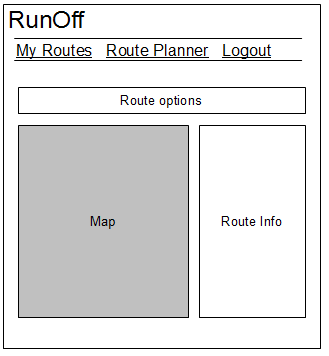
\includegraphics[scale=1]{img/webmockup1.png}
\end{figure}

Four views, which should constitute an \ac{MVP}, were planned for this sprint:
\begin{itemize}
 \item {Route Designer} (Only available when logged in)
 \item {Route Overview} (Only available when logged in)
 \item {User Registration}
 \item {User Log In}
\end{itemize}

The route overview should be a simple listing of the routes the current user has created, with a summary of the information available for that route, as well as a link to modify each route. The registration and log in views should be simple \ac{HTML} forms.

The route planner is where most of the work should be done. The planner should display a map, and the following controls on the map:

\begin{itemize}
 \item Clicking the map should add a waypoint
 \item Clicking and dragging a waypoint should move it
 \item Right-clicking a waypoint should delete it
\end{itemize}

After each of these actions has been performed, a route should be created, snapping the route to paths and pavements, as well as allowing users to see useful information, such as the total distance and topography of the route.

Additionally, the planner should expose various controls separate from the map itself, including the ability to name the route, mark it as a round-trip (Using the first waypoint as both start and end of the route) as well as submitting the route and saving it on the server.

\subsection{Database Model}

\begin{figure}[ht]
 \caption{Sprint 1 Database Model}
 \label{fig:sprint1-db-model}
 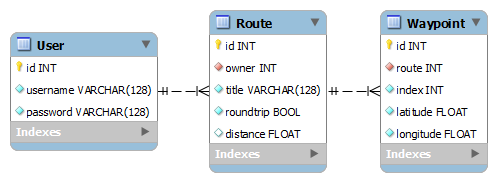
\includegraphics[scale=0.5]{img/sprint1db.png}
\end{figure}

\subsection{Implementation}

\begin{figure}[ht]
 \caption{Sprint 1 Webpage}
 \label{fig:sprint1-web-screen}
 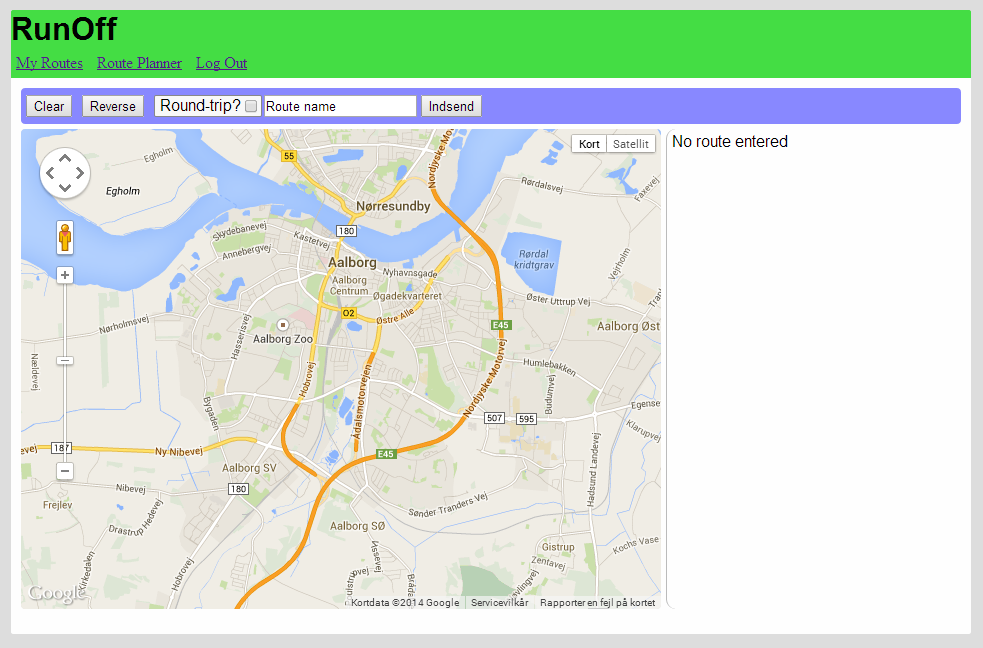
\includegraphics[width=\textwidth]{img/webplanner1.png}
\end{figure}

\subsection{Tests}
